\documentclass[11pt]{article}
\usepackage[dvipsnames]{xcolor}
\usepackage[T1]{fontenc}
\usepackage{mathtools}
\usepackage[french]{babel}
\usepackage{amsmath,amssymb,amsthm}
\usepackage{framed}
\usepackage{lmodern}
\usepackage{utils}
\usepackage{pdfpages}
\usepackage{irif}
\usepackage{listings}
\usepackage{listingsutf8}

\definecolor{codegreen}{rgb}{0,0.6,0}
\definecolor{codegray}{rgb}{0.5,0.5,0.5}
\definecolor{codepurple}{rgb}{0.58,0,0.82}
\definecolor{backcolour}{rgb}{0.96,0.96,0.95}
\newcommand*{\pmZpmZ }{p^m\Z \x p^m\Z}
\newcommand*{\ZZpmZ}{\Z^2/\pmZpmZ}
\newcommand*{\ZZnZ}{\Z^2/\nZnZ}



\lstdefinestyle{mystyle}{
    backgroundcolor=\color{backcolour},
    commentstyle=\color{codegreen},
    keywordstyle=\color{magenta},
    numberstyle=\tiny\color{codegray},
    stringstyle=\color{codepurple},
    breakatwhitespace=false,
    breaklines=true,
    captionpos=b,
    keepspaces=true,
    numbers=left,
    numbersep=5pt,
    showspaces=false,
    showstringspaces=false,
    showtabs=false,
	extendedchars=true,
    tabsize=4,
	basicstyle=\ttfamily,
  	mathescape,
	inputencoding=utf8/latin1,
	literate=%
		{é}{{\'e}}{1}%
		{è}{{\`e}}{1}%
		{à}{{\`a}}{1}%
		{ç}{{\c{c}}}{1}%
		{œ}{{\oe}}{1}%
		{ù}{{\`u}}{1}%
		{É}{{\'E}}{1}%
		{È}{{\`E}}{1}%
		{À}{{\`A}}{1}%
		{Ç}{{\c{C}}}{1}%
		{Œ}{{\OE}}{1}%
		{Ê}{{\^E}}{1}%
		{ê}{{\^e}}{1}%
		{î}{{\^i}}{1}%
		{ô}{{\^o}}{1}%
		{û}{{\^u}}{1}%
		{ë}{{\¨{e}}}1
		{û}{{\^{u}}}1
		{â}{{\^{a}}}1
		{Â}{{\^{A}}}1
		{Î}{{\^{I}}}1
}

\lstset{style=mystyle}

\begin{document}
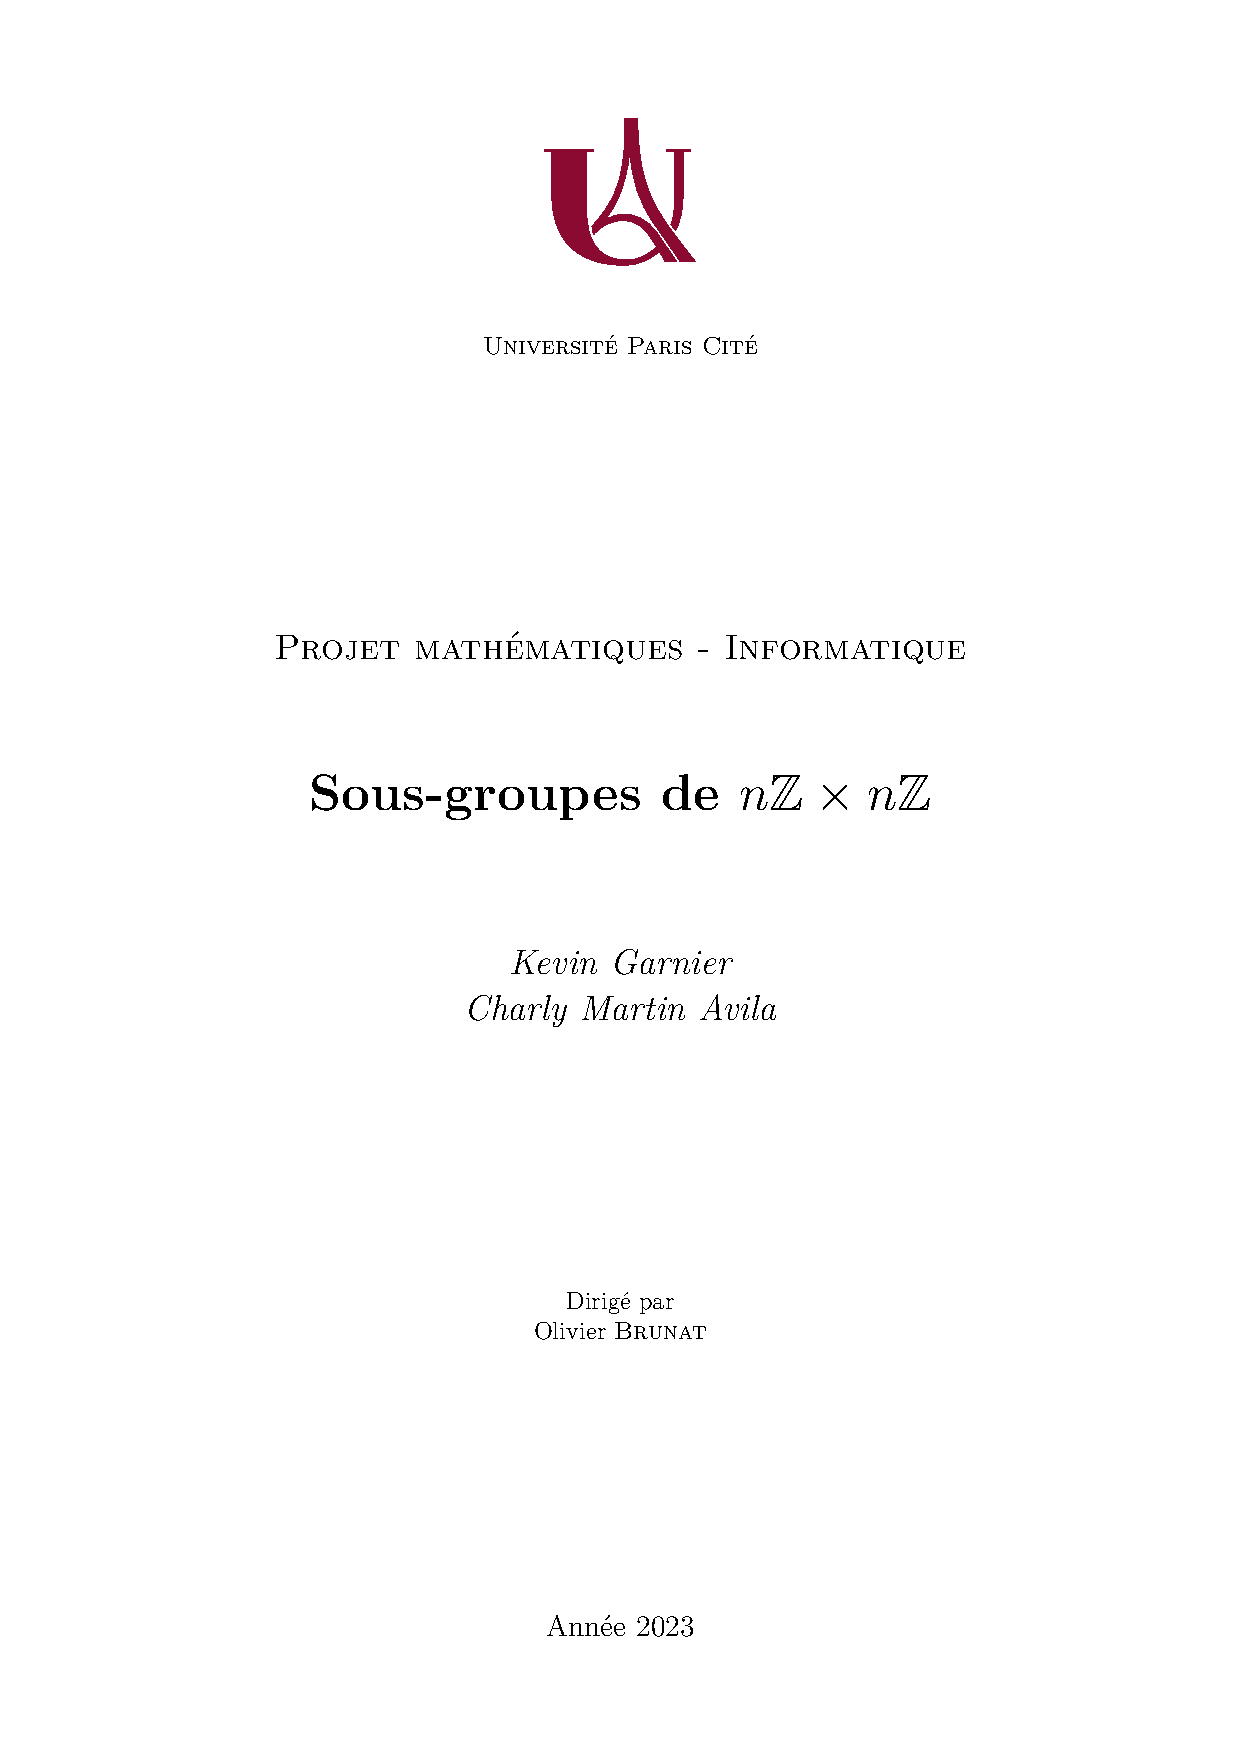
\includepdf{title.pdf}
\hfill
\newpage
\tableofcontents

%%%%%%%%%%%%%%%%%%%%%%%%%%%%%%%%%%%%%%%%%%%%%%%%%%%%%%%%%%%%%%%%%%%%%%%%
\newpage
\section{Introduction}
Il est très facile de décrire tous les sous-groupes d'un groupe cyclique
d'ordre $n$ : il y en a exactement un par diviseur positif de $n$.
Pourtant, étonnamment, décrire tous les sous-groupes d'un groupe abélien
est en général un problème difficile.\\
Dans ce projet, nous nous se proposons de considérer cette question pour le groupe $\ZZ$ qui,
de nos jour n'a pas l'air d'avoir été traitée.

D'un point de vue théorique, nous mettrons en avant la générations et la caractérisations de \\
sous-groupes grâce aux vecteurs colonne des matrices à coefficients entier et en particulier aux formes
normales de Hermite. Nous montrerons aussi une formule permettant de les compter.

D'un point de vue pratique, nous créerons un programme \textsc{OCaml} capable de générer les\\
sous-groupes de $\ZZ$ ainsi que leur treillis à partir d'un entier donné en paramètres.

%%%%%%%%%%%%%%%%%%%%%%%%%%%%%%%%%%%%%%%%%%%%%%%%%%%%%%%%%%%%%%%%%%%%%%%%
\newpage
\section{Quelques simplifications du problème}
%- - - - - - - - - - - - - - - - - - - - - - - - - - - - - - - - - - - -
\subsection{Décomposition de $n$ en éléments irréductibles}\label{theoreme_chinois}

Nous pouvons tout d'abord simplifier le problème aux cas où $n = p^m$ avec $p$ un nombre premier
et $m \in \N$. En effet la proposition suivante nous garantie que le résultat est isomorphe
\begin{proposition}
	Soit $n = \prod\limits_i^k p_i^{\alpha_i}$, avec $p_i$ des nombres premiers, alors
	$$(\ZZ) \isom \prod_i^k(\Z/p_i^{\alpha_i}\Z)^2$$
\end{proposition}

\begin{proof}
	Soit $n = \prod\limits_i^k p_i^{\alpha_i}$. Par le théorème des restes chinois, on a
	$$ \ZnZ \isom (\Z/p_i^{\alpha_i}\Z) \x \cdots \x (\Z/p_i^{\alpha_i}\Z)$$
	En particulier,
	\begin{equation*}
		\begin{split}
			\ZZ & \isom
			(\Z/p_i^{\alpha_i}\Z) \x \cdots \x (\Z/p_i^{\alpha_i}\Z) \x (\Z/p_i^{\alpha_i}\Z) \x \cdots \x (\Z/p_i^{\alpha_i}\Z)\\
			& \isom (\Z/p_i^{\alpha_i}\Z)^2 \x \cdots \x (\Z/p_i^{\alpha_i}\Z)^2
		\end{split}
	\end{equation*}
\end{proof}

En pratique, pour décomposer en entier en facteurs irréductibles, nous avons utilisé la procédure de
\textsc{$\rho$-Pollard} pour obtenir un diviseur de $n$:
\begin{lstlisting}
fonction rho_pollard P n x y k i d
    Si d <> 1:
        Retourne d
    Sinon:
        x = P(x) mod n
        d = pgcd(|y - x|, n)
        Si i = k:
            Alors Retourne rho_pollard loop P n x x 2k (i + 1) d
        Sinon Retourne rho_pollard P n x y k (i + 1) d
\end{lstlisting}
Puis nous répétons la procédure jusqu'à que les diviseurs soient premier.\\
En triant et en regroupant les nombres premier, nous obtenons donc les différents $p^{\alpha_i}_i$.\\
Dans notre implémentation, $P(X) = X^2 - 1$ et $n$ n'est pas premier.
%TODO : Ajout algo test primarite ?
%- - - - - - - - - - - - - - - - - - - - - - - - - - - - - - - - - - - - - -
\newpage
\subsection{Simplification des sous-groupes}\label{simp_ss_gr}

\begin{proposition}
	$$\Z^2/n\Z \x n\Z \isom \ZZ $$
\end{proposition}
\begin{proof}
	Soit \app{\varphi}{\Z^2}{\ZZ}{(a,b)}{(\bar a, \bar b)}
	$\varphi$ est surjective par définition de la classe d'équivalence de a et b.
	Montrons que $\ker \varphi = n\Z \x n\Z$.

	\begin{equation*}
		\begin{split}
			&(a,b) \in \ker \varphi \\
			&\text{ssi } \varphi(a,b) = (\bar 0, \bar 0)\\
			&\text{ssi } (\bar a, \bar b) = (\bar 0, \bar 0)\\
			&\text{ssi } \bar a = \bar 0 \text{ et } \bar b = \bar 0\\
			&\text{ssi } a \in n\Z \text{ et } b \in n\Z\\
			&\text{ssi } (a,b) \in  n\Z \x n\Z
		\end{split}
	\end{equation*}
	Ainsi par le premier théorème d'isomorphisme, on a
	$$\Z^2/n\Z \x n\Z \isom \ZZ $$
\end{proof}
Ainsi le problème se résout à trouver les sous-groupes $G$ de $\Z^2$ tels que
$H = \matsqr{a}{c}{b}{d}$\\
et
$n\Z \x n\Z \subseteq G = \gen{\vectcolsqr{\bar a}{\bar b}, \vectcolsqr{\bar c}{\bar d}}$

%%%%%%%%%%%%%%%%%%%%%%%%%%%%%%%%%%%%%%%%%%%%%%%%%%%%%%%%%%%%%%%%%%%%%%%%%%%%%%
\newpage
\section{Matrices à coefficients entier et forme normales de Hermite}
Nous avons vu dans la section précédente qu'il était possible de caractériser les sous-groupe de
$\ZZ$ par une matrice $H = \matsqr{a}{c}{b}{d}$. Cependant, ces matrices ne sont pas uniques. C'est
pourquoi, nous allons utiliser les formes normales d'Hermite.
Énonçons d'abord une proposition les matrices à coefficients entier qui nous sera forte utile par la suite.
%problème section précédente, il existe un nombre important de matrice similaire i.e qui
%engendre le même sous groupe
%- - - - -- - - - - - - - - - - - - - - - - - - - - - - - - - - - - - - - -
\subsection{Matrices à coefficients entier}
\begin{proposition}\label{ima_imaq}
	Soient $A \in \M_{m,n}(\Z)$ et $Q \in \GL_n(\Z)$, alors
	$$\im AQ = \im A$$
\end{proposition}
\begin{proof}
	Soit $y \in \im AQ$, il existe $x \in \Z^n$ tel que $y = AQx$. Or,
	\begin{align*}
		         & y = AQx     \\
		\implies & y = A(Qx)   \\
		\implies & y \in \im A
	\end{align*}
	Donc $\im AQ \subseteq \im A$.
	Soit $y \in \im A$. Il existe $x \in \Z^n$ tel que $y = Ax$.\\
	Cherchons $z \in \Z^n$ tel que $y = Ax = AQz$
	\begin{align*}
		         & Ax = AQz                                     \\
		\implies & A(x) = A(Qz)                                 \\
		\implies & x = Qz                                       \\
		\implies & \inv Q x = z \text{ (car $B \in \GL_n(\Z)$)}
	\end{align*}
	Donc il existe bien un $z \in \Z^n$ tel que $ABz = y$. Donc $y \in \im AQ$.\\
	D'où $\im AQ = \im A$

\end{proof}

%- - - - - - - - - - - - - - - - - - - - - - - - - - - - - - - - - - - - -
\newpage
\subsection{Formes normales de Hermite}
Nous allons désormais énoncer la définition de la forme normale de Hermite.
\begin{definition}
	Soit $A \in \M_{m,n}(\Z)$. Alors il existe une unique matrice échelonnée
	réduite suivant les colonnes $H \in \M_{m,n}(\Z)$ telle qu'il existe $Q \in \GL_n(\Z)$
	avec $H = AQ$. La matrice $H$ s'appelle la forme normale de Hermite de A.
\end{definition}

\begin{proof}
	Nous supposerons l'unicité admise, l'algorithme suivant nous montre son existence.
	\begin{lstlisting}
Fonction hermite_aux($A$, $i$):
	Pour chaque $j$ allant de $i$ à $m$ :
		Si i = j :
			Si $a_{ij} < 0$ : réaliser l'opération $C_j \leftarrow -C_j$
		Sinon :
			Si $a_{ij}$ < 0 : réaliser l'opération $C_j \leftarrow -C_j$
			$k,r$ = div_euclide($a_{ij}$, $a_{ii}$)
			réaliser l'opération $C_j \leftarrow C_j - kC_i$
	Si $\forall i < j <= m, a_{ij} = 0$ :
		Réduire à gauche du pivot
		Retourner A
	Sinon
	$d_{k} = \min(\Set*{a_{ij}}{i <= j <= n a_{ij} \ne 0})$
	Permuter $C_k$ avec $C_i$
	hermite_aux($A$, $i$)

Fonction hermite(A) :
	Pour chaque $i$ allant de A à $n$ :
		$d_{k} = \min(\Set*{a_{ij}}{i <= j <= n a_{ij} \ne 0})$
		Si $d = None$ :
			Continuer boucle
		Sinon :
			Permuter $C_k$ avec $C_i$
			$A$ = hermite_aux($A$, $i$)
	vérifier signe des pivots de $A$
	Retourner $A$


\end{lstlisting}

	Montrons la terminaison de l'algorithme.
	La fonction \texttt{hermite\_aux} se repose sur l'algorithme \\d'euclide. En effet, pour tout $i < j < m$, on réalise la
	division euclidienne de $a_{ij}$ par $a_{ii}$.\\
	Si à la fin de la boucle il existe $j$ tel que
	$a_{ij} < a_{ii}$, alors on recommence en permutant $C_j$ et $C_i$ et $a_{ij}$ devient notre nouveau pivot.\\
	Ainsi, par la correction de l'algorithme d'Euclide, il existe un rang $N$ où tous les $a_{ij}$ avec $j> i$ sont tous nuls.
	Ainsi la fonction \texttt{hermite\_aux} se termine. La fonction \texttt{hermite} étant seulement une boucle, elle se termine également.
	Donc l'algorithme se termine bien.

	Montrons la correction de l'algorithme.	La fonction hermite\_aux se repose sur l'algorithme\\
	d'Euclide en utilisant des opérations élémentaires sur les matrices.\\
	Par la correction de l'algorithme d'Euclide, nous pouvons en déduire que pour tout $j > i$, $a_{ij} = 0$.\\
	De plus, avant de retourner, on réalise la division euclidienne des $a_{ij}$ par $a_{ii}$ avec $0 < j < i$.\\
	Donc les $a_{ij}$ sont les restes des divisions euclidiennes et sont donc réduit au maximum.\\
	On réalise ces opération sur toutes les lignes sans jamais revenir sur les lignes précédentes.
	Enfin, on vérifie le signe de pivot et on change la colonne de signe si nécessaire.\\
	Ainsi la matrice obtenue est bien échelonnée réduite,
	il s'agit donc d'une forme normale de Hermite, ce qui prouve donc son existence.

\end{proof}

\begin{example}
	\begin{equation*}
		\begin{split}
			A =
			\begin{pmatrix}
				2  & 1  \\
				4  & 10 \\
				5  & 13 \\
				13 & 12
			\end{pmatrix}
			\overset{C_2 \leftrightarrow C_1}{\longrightarrow}
			\begin{pmatrix}
				1  & 2  \\
				10 & 4  \\
				13 & 5  \\
				12 & 13
			\end{pmatrix}
			\overset{C_2 \leftarrow C_2 - 2C_1}{\longrightarrow}
			\begin{pmatrix}
				1  & 0   \\
				10 & -16 \\
				13 & 3   \\
				12 & -14
			\end{pmatrix}
			\overset{C_2 \leftarrow - C_2}{\longrightarrow}
			\begin{pmatrix}
				1  & 0  \\
				10 & 16 \\
				13 & -3 \\
				12 & 14
			\end{pmatrix} = H
		\end{split}
	\end{equation*}

\end{example}
\begin{remark}
	Il existe des algorithmes beaucoup plus efficace pour calculer la forme normale de Hermite comme
	l'algorithme de de Domich \& Ai (1989) qui réalise les calculs modulo le déterminant de $A$ ou
	l'algorithme de Micciancio-Warinshi. Cependant ces algorithmes étant plus ou moins compliqué, le choix ici
	a été de faire nous même un algorithme à partir	de la méthode naïve employée lors du calcul de la forme normale de
	Hermite à la main.
\end{remark}
\begin{definition}
	Soient $A \in \M_{m,n}$, $B \in \M_{m,p}$ deux formes normales de Hermite
	$$A \sim B \text{ ssi les colonnes non nulles de } A
		\text{ sont les mêmes que les colonnes non nulles de } B.$$
\end{definition}
Nous allons énoncer quelques résultats utiles des formes normales de Hermite.
Tout d'abord, la proposition suivante nous permettra de réduire nos forme de matrices dont les colonnes
génèrent un sous groupe de $\Z^2$
\begin{proposition}\label{ima_imh}
	Soit $A \in \M_{m,n}(\Z)$ et soit $H$ sa forme normale d'Hermite. Alors,
	$$\im A = \im H$$
\end{proposition}

\begin{proof}
	C'est une application de la proposition \ref{ima_imaq} avec $H= AQ$ avec $Q \in \GL_n(\Z)$

\end{proof}

Ainsi les colonnes de la forme normale de Hermite $H$ d'une matrice $A$ génèrent le même
sous-groupe que les colonnes de $A$.\\
Nous n'avons donc plus qu'à trouver des matrices de la forme
$H = \matsqr{a}{0}{b}{c}$ telle que
$$n\Z \x n\Z \subseteq \gen{\vectcolsqr{\bar a}{b},\vectcolsqr{0}{\bar c}}$$

\begin{proposition}\label{ha_hb_ssi_ima_imb}
	Soient $A,B \in \M_{m,n}(\Z)$.\\
	Soit $H_A$ (resp. $H_B$) la forme normale de Hermite de $A$ (resp. $B$). Alors,
	$$ H_A = H_B \ssi \im A = \im B$$
\end{proposition}

\begin{proof}
	Supposons que $H_A = H_B$.	Par la proposition \ref{ima_imh}, on a
	$$\im A = \im H_A = \im H_B = \im B$$
	Réciproquement, supposons que $\im A = \im B$. Par la proposition \ref{ima_imh}, on a
	$$\im A = \im H_A = \im H_B = \im B$$
	Donc les vecteurs colonnes de $H_A$ qui génèrent $\im H_A$ sont les mêmes que ceux de
	$H_B$ qui génèrent $\im H_B$, d'où $H_A = H_B$

\end{proof}

Cette proposition nous affirme donc qu'en traitant seulement
les formes normales de Hermite, nous pourrons générer tous les sous-groupes de $\Z^2$

La proposition suivante, va nous être utile pour trouver la bonne forme des matrices de Hermite
ainsi que la génération du treillis.

\begin{proposition}\label{guh_g_ssi_a_sim_b}
	Soient $A,B \in \M_{m,n}$ deux formes normales de Hermite et soit $G$ (resp. $H$) le
	groupe engendré par les colonnes de $A$ (resp. $B$). Alors,
	$$G \cup H = G \ssi hermite(A | B) \sim A$$
	où $hermite(A|B)$ est la forme normale de hermite de la matrice augmentée $(A | B)$.
\end{proposition}

\begin{proof}
	Supposerons que $G \cup H = G$. Alors $ H \subseteq G$.Donc
	$$\forall x \in H \cma  \ex y \in G \cma \ex \lambda \in \Z \cma x = \lambda y$$
	En particulier la base de $H$ est une combinaison linéaire de la base de $G$. D'où
	$$hermite(A | B) = (A | 0) \sim A$$
	Réciproquement, soit $hermite(A | B) \sim A$. Alors par définition de la relation
	d'équivalence,\\
	$hermite(A | B) = (A | 0)$. Ainsi les colonnes de B sont des combinaisons linéaire des
	colonnes de $A$,\\
	\cad \, la base de $H$ est une combinaison linéaire de la base de $G$.
	$$\text{D'où } H \subseteq G \text{ et } G \cup H = G$$
\end{proof}

Nous avons désormais tous les outils à notre disposition pour
démontrer la forme voulue des matrices ainsi que la formule permettant de compter le nombre
de sous-groupe de $\ZZnZ$

%%%%%%%%%%%%%%%%%%%%%%%%%%%%%%%%%%%%%%%%%%%%%%%%%%%%%%%%%%%%%%%%%
\newpage
\section {Génération et énumération des sous-groupes}
Nous allons voir dans cette section la forme des matrices dont les vecteurs colonne génèrent
les sous-groupes de $\ZZnZ$, la formule permettant de les compter ainsi que quelques propositions
sur leurs caractéristiques. Nous avons montré dans la section \ref{theoreme_chinois} que nous pouvons nous
restreindre aux cas où $n = p^m$ avec $p$ un nombre premier et $m \in \N$.\\
Ainsi dans cette section, nous supposerons que $n = p^m$.

%- - - - - - - - - - - - - - - - - - - - - - - - - - - - - - - -
\subsection{Génération des sous-groupes}
Commençons tout d'abord par montrer la forme des matrices dont les vecteurs colonne génèrent
les sous-groupes de $\ZZpmZ$. Dans la section \ref{simp_ss_gr}, nous avons montré que les
sous-groupes de $\Z^2$ recherché sont les sous groupes $G$ tels que
$\pmZpmZ \subseteq G$, \cad
$$ G \cup \pmZpmZ = G$$
Par la proposition \ref{guh_g_ssi_a_sim_b}, cela revient à trouver les
matrices $H = \begin{pmatrix}
		\alpha & 0      \\
		\beta  & \gamma
	\end{pmatrix}$
telles que $$(H | Mat(\pmZpmZ)) =
	\begin{pmatrix}
		\alpha & 0      & p^m & 0   \\
		\beta  & \gamma & 0   & p^m
	\end{pmatrix}
	\sim	\begin{pmatrix}
		\alpha & 0      \\
		\beta  & \gamma
	\end{pmatrix}
	= H
$$

\begin{theorem}
	Les seules matrices dont les colonnes génèrent un sous-groupe de $\ZZpmZ$
	sont les matrices de la forme
	$$H =
		\begin{pmatrix}
			p^a & 0   \\
			j   & p^b
		\end{pmatrix}
		\text{avec $a \le m$, $b \le m$ et $j < p^b$}
	$$
	$$ \text{ ou }$$
	$$ H =\begin{pmatrix}
			p^a  & 0   \\
			jp^k & p^b
		\end{pmatrix}
		\text{avec $a \le m$, $b \le m$, $k \le m$ et $j < p^{b - k}$}
	$$

\end{theorem}
\begin{proof}
	Montrons tout d'abord que ces matrices sont les seules qui génèrent les sous-groupe de $\ZZ$.\\
	Supposons qu'il existe $H,H'$ deux formes normales de Hermite qui génèrent $G$ un sous-groupe
	de $\ZZ$. Alors, on a $\im H = \im H'$ et par la proposition \ref{ha_hb_ssi_ima_imb}, $H = H'$.\\
	Nous pouvons donc créer une classe d'équivalence pour la relation $\sim$ où la matrice de hermite
	est la représentante de ces classes.\\
	Montrons désormais l'existence de telles matrices.\\
	Soit
	$H = \begin{pmatrix}
			a & 0 \\
			b & c
		\end{pmatrix}$
	On cherche à réaliser des operations élémentaires telles que
	\begin{equation*}
		A = \begin{pmatrix}
			\alpha & 0      & p^m & 0   \\
			\beta  & \gamma & 0   & p^m
		\end{pmatrix}
		\longrightarrow
		\begin{pmatrix}
			\alpha & 0      & 0 & 0 \\
			\beta  & \gamma & 0 & 0
		\end{pmatrix}
	\end{equation*}
	Annuler $a_{1\,3} = a_{2\,4} = p^m$ nécessite les conditions suivante sur $\alpha$ et $\beta$ :
	$$\begin{cases*}
			\alpha = p^a \text{ avec } a \le m\\
			\gamma = p^b \text{ avec } a \le m\\
		\end{cases*}$$
	Nous pouvons donc réaliser les opérations $C_3 \leftarrow C_3 -p^{m-a}C_1$ et
	$C_4 \leftarrow C_4 -p^{m-b}C_2$. Ceci nous donne donc :
	\begin{equation*}
		\begin{pmatrix}
			\alpha & 0      & p^m & 0   \\
			\beta  & \gamma & 0   & p^m
		\end{pmatrix}
		\overset{C_3 \leftarrow C_3 -p^{m-a}C_1 }{\overset{ C_4 \leftarrow C_4 -p^{m-b}C_2}{\longrightarrow}}
		\begin{pmatrix}
			\alpha & 0      & 0             & 0 \\
			\beta  & \gamma & -p^{m-a}\beta & 0
		\end{pmatrix}
	\end{equation*}
	Nous cherchons désormais $\beta$ tel que $\divided{p^b}{\beta p^{m-a}}$.\\
	Tout d'abord, par la définition de la forme normale de Hermite, $\beta< p^b$.\\
	Nous pouvons isoler deux cas en fonction de $a$ et $b$ :\\
	\begin{itemize}
		\item Si $a + b \le m$, alors $b \le m - a$ et $\divided{p^b}{p^{m-a}}$ et
		      donc $\divided{p^b}{\beta p^{m-a}}$.\\
		\item Sinon $m \le a + b \le 2m \implies 0 \le a + b -m \le n$.\\
		      On pose $k = a + b -m$ et on a donc $0 \le k \le m$.\\
		      On pose $\beta = ip^k$ avec $0 \le i < p^{b - k}$. On a bien
		      $\fa i \cma \beta = ip^k < p^b$.\\
		      De plus $\divided{p^b}{ip^kp^{m-a}}$ car $\divided{p^b}{p^kp^{m-a}}$
		      car $b = k + m - a$
	\end{itemize}
	Ainsi, dans les deux cas, nous pouvons annuler $a_{2\,3}$ et nous obtenons bien la matrice
	suivante en faisant l'operations élémentaire.
	$\begin{pmatrix}
			\alpha & 0      & 0 & 0 \\
			\beta  & \gamma & 0 & 0
		\end{pmatrix}$.\\
	Dans le premier cas, nous obtenons en posant $j = \beta < p^b$
	\begin{equation*}
		\begin{pmatrix}
			p^a & 0   & 0 & 0 \\
			j   & p^b & 0 & 0
		\end{pmatrix}
		\sim
		\begin{pmatrix}
			p^a & 0   \\
			j   & p^b
		\end{pmatrix}
	\end{equation*}
	Dans le deuxième cas, nous obtenons en posant $j = i < p^{b-k}$
	\begin{equation*}
		\begin{pmatrix}
			p^a  & 0   & 0 & 0 \\
			jp^k & p^b & 0 & 0
		\end{pmatrix}
		\sim
		\begin{pmatrix}
			p^a  & 0   \\
			jp^k & p^b
		\end{pmatrix}
	\end{equation*}

	Ce qui démontre bien l'existence de ces matrices.

\end{proof}

\begin{corollary}
	Soit la suite $\suit{A}{k}{0 \le k \le n}$ telle que
	\begin{equation*}
		\begin{split}
			&A_0 = \Set*{(a,b)}{ a + b \le m}\\
			&A_k = \Set*{
				(a,b)}{
				\begin{aligned}
					 & a \le m, b \le m \\
					 & a + b = m + k
				\end{aligned}
			}
		\end{split}
	\end{equation*}
	Alors, l'ensemble des matrices du théorème, \cad, les matrices dont les colonnes
	génèrent les sous-groupes de $\ZZpmZ$ est
	$$M = \bigsqcup_{k = 0}^mM_k$$
	où
	\begin{equation*}
		M_k = \Set*{
			\begin{pmatrix}
				p^a  & 0   \\
				jp^k & p^b
			\end{pmatrix}
		}{
			\begin{aligned}
				 & (a, b) \in A_k      \\
				 & 0 \le j < p^{b - k}
			\end{aligned}
		}
	\end{equation*}
\end{corollary}

\begin{proposition}
	%projection <\pi(alpha, j), \pi(0, beta)
\end{proposition}

\newpage
\begin{example}[Cas pour $n = 2$]
	On a $n = 2 = 2^1$ donc $m = 1$.\\
	Calculons les matrices appartenant à $M_0 = \Set*{
			\begin{pmatrix}
				p^a & 0   \\
				j   & p^b
			\end{pmatrix}
		}{
			\begin{aligned}
				 & (a, b) \in A_0  \\
				 & 0 \le j < p^{b}
			\end{aligned}
		}$\\
	On a $A_0 = \Set*{(a,b)}{a + b \le 1} = \set{(0,0), (0,1), (1, 0)}$.
	Ainsi
	\begin{equation*}
		M_0 = \set{
			\matsqr{1}{0}{0}{1}, \matsqr{1}{0}{0}{2}, \matsqr{1}{0}{1}{2}, \matsqr{2}{0}{0}{1}
		}
	\end{equation*}
	Calculons les matrices appartenant à $M_1 = \Set*{
			\matsqr{2^a}{0}{2j}{2^b}
		}{
			\begin{aligned}
				 & (a, b) \in A_1      \\
				 & 0 \le j < 2^{b - 1}
			\end{aligned}
		}$.\\
	On a $A_1 = \Set*{
			(a,b)}{
			\begin{aligned}
				 & a \le 1, b \le 1 \\
				 & a + b = 2
			\end{aligned}
		} = \set{(1,1)}$. Ainsi
	$$M_0 = \set{\matsqr{2}{0}{0}{2}}$$
%Ajouter correspondances avec les sous-groupes de \ZZ
\end{example}

%proposition sur le cardinal
%card sous-groupe = p^{a + b}
%- - - - -- - - - - -- - - - - - -- - - - - - - -- -- - - - - - - - - - - - - -
\subsection{Énumération des sous-groupes}
%preuve sur le calcul du nombre de sous-groupe
%%%%%%%%%%%%%%%%%%%%%%%%%%%%%%%%%%%%%%%%%%%%%%%%%%%%%%%%%%%%%%%%%%%%%%%%%%%%%%
\newpage
\section{Génération du treillis}
%Algorithme génération du treillis
%Choix de .dot et graphivz

%%%%%%%%%%%%%%%%%%%%%%%%%%%%%%%%%%%%%%%%%%%%%%%%%%%%%%%%%%%%%%%%%%%%%%%%%%%%%%%%
\newpage
\section{Quelques résultats}
%- - - - - - - - - - - - - - - - - - - - - - - - -- - - - - - - - -- - - - - -
\subsection{Pour n = 2}
%pour n = 2
%- - - - - -- - - - - - - - - - - - - - - - - - - - - - - - -- - - - - - -- - -
\subsection{Pour n = 4}
% pour n = 4
%- - - - - - - - - - - - - - - - - - - - - - - - - - - - - - - - - - - - - - -
\subsection{Pour n = 20}
% pour n = 20

%nombre de sous-groupes + treillis .dot
%%%%%%%%%%%%%%%%%%%%%%%%%%%%%%%%%%%%%%%%%%%%%%%%%%%%%%%%%%%%%%%%%%%%%%%%%%%%%%
\newpage
\section{Bibliographie}
\begin{enumerate}

	\item[[\,1\!\!]] COSTE Michel, \textit{Algèbre linéaire sur les entiers}, Mars 2018
	\item[[\,2\!\!]] \textbf{TODO livre algo}
	\item[[\,3\!\!]] PERNET Clément, \textit{Calcul de formes normales matricielles: de
		      l'algorithmique à la mise en \\pratique}, Séminaire SIESTE, ENS-Lyon, 12 février 2013
	\item[[\,4\!\!]] BERHURY Grégory, \textit{Algèbre le grand combat : Cours et exercices}, $2^e$ édition.\\
	      Paris : Calvage \& Mounet, 2020. 1215 p. (Mathématiques en devenir)
\end{enumerate}
\end{document}
